\chapter{Detekcia útokov na SCADA systémy}
\tab V nasledujúcej kapitole sa zameriam na možnosti detekcie rôznych typov útokov popísaných v kapitole \ref{bezpecnost} spolu s popisom ochrany systémov a sietí pred nimi. \par
Na obrázku \ref{attack} je možné vidieť model jednoduchého kybernetického útoku.
\begin{figure}[h]
    \centering
    \scalebox{0.7}{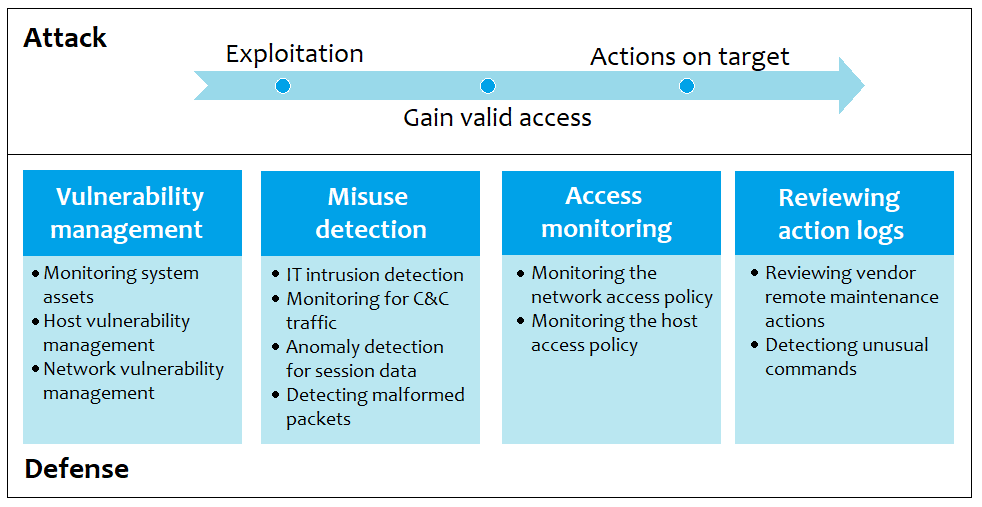
\includegraphics{attack}}
    \caption{Model jednoduchého kyber-útoku}
\label{attack}
\end{figure}
Myšlienka za týmto modelom je, že väčšina útokov začína s využitím zraniteľností danej siete kvôli získaniu prístupu do systému. Keď sa raz útočník dostane "dnu", snaží sa získať oprávnenia na získanie platného prístupu k jednotlivým prvkom systému. Akonáhle má čo potreboval, vykoná kroky potrebné na dosiahnutie svojho cieľa, napríklad na prepnutie alebo vypnutie rôznych častí siete. \par
Stratégia detekcie pozostáva zo štyroch častí:
\begin{itemize}
\item Kontrola a riadenie zraniteľností systému - nájdenie a odstránenie zraniteľných miest skôr ako môžu byť využité útočníkom.
\item Detekcia zneužitia - detekovanie napadnutia systému.
\item Monitorovanie prístupu - detekovanie neoprávnených alebo škodlivých akcií s platnými povereniami.
\item Kontrola logovacích záznamov - zisťovanie akcií s platnými povereniami, ktoré sú škodlivé alebo proti bezpečnostným pravidlám.
\end{itemize}
Model na obrázku \ref{attack} je veľmi zjednodušený. Skutočný útok nemusí byť takto priamočiarý. Útočníci môžu napríklad potrebovať nájsť niekoľko zraniteľných miest v systéme, kým sa im ich podarí využiť a získať platný prístup. Môžu tiež vykonávať rôzne akcie na preskúmanie vlastností danej siete alebo môžu úplne preskočiť fázu hľadania zraniteľných miest, ak už majú k dispozícií platne autentizačné údaje\cite{Security}\cite{IoTSec}.

\section{Kontrola a riadenie zraniteľností systému}
\tab Aktivity kontroly a riadenia zraniteľností sú iba preventívne opatrenia pre systém. Pokúšajú sa nájsť a opraviť zraniteľné miesta a zadné vchody (backdoor) do systému, skôr ako sú odhalené útočníkmi. Ako také zmierňujú väčšinu hrozieb s výnimkou vnútorných, ktoré sa využívajú iba s platnými povereniami. \par
Sú zamerané na hľadanie chýb v systéme a na ich opravu. V OT sieťach je zabezpečenie veľmi závislé od architektúry daného systému. Ak sa v sieti využívajú staršie zariadenia, je potrebné hľadať zraniteľné miesta priamo v architektúre, nakoľko nie je možné sa spoliehať iba na zabezpečenie daného zariadenia. \par
Na efektívnu kontrolu je potrebné mať podrobný prehľad o pripojených zariadeniach a o ich konfigurácií. Tieto informácie uľahčujú nájsť a opravit slabé miesta a zadné vchody do systému. Základné aktivity na kontrolu systému sú:
\begin{itemize}
\item Sledovať/reagovať na novo-pripojené zariadenia do siete
\item Monitorovať prístupy k portom a MAC adresy na jednotlivých prepínačoch
\item Použiť alarm pri pripojení nového zariadenia
\item Odstrániť neautorizovaných hostov
\end{itemize}
Alarmy na nové zariadenia môžu byť využívané za pomoci aktívneho alebo pasívneho skenovania siete. Aktívne skenovanie môže byť vykonávané za pomoci nástrojov ako {\tt nmap} a pasívne sledovaním sieťovej prevádzky. \par
Avšak vykonávanie takejto aktivity vyžaduje zoznam povolených zariadení, ktoré majú oprávnenie sa pripojiť do SCADA systému, aby mohli byť neoprávnené jednoduchšie detekovateľné. Na začiatku monitorovania ale väčšinou obdobný zoznam nie je plne k dispozícií a tak je potrebné aby sa postupne vytváral spolu s monitorovacou aktivitou. \par
Okrem zoznamu je tiež potrebné dodržiavať isté pravidlá pri pripájaní nového zariadenia. To môže byť riešené podrobným registračným procesom, ktorý pomože analytikom overiť, že zariadenie má oprávnenie na vstup do systému\cite{Security}.

\section{Detekcia zneužitia}
\tab Aktivity na detekovanie zneužitia hľadajú v komunikácií znaky známych útokov. V IT sfére bolo za týmto účelom vyvinutých veľa senzorov a sónd. Môžu byť naviazané na hostiteľa, ako napríklad rôzne antivírové programy, alebo priamo na sieť, ako napríklad rôzne systémy na detekciu narušenia siete. \par
Pôvodne boli senzory využívané na detekciu správnosti autentizačných údajov a podpisov. Používané pravidlá boli spisované priamo výrobcom daného senzoru na základe poznatkov o zaznamenaných útokoch. Na dosiahnutie spoľahlivej úrovne detekcie boli potrebné desaťtisíce pravidiel, ktoré museli byť pravidelne aktualizované. Moderné systémy na detekciu narušení doplňujú tento prístup o využitie inteligentných algoritmov, pomocou ktorých je možné odhaliť niekoľko rôznych tried útokov. Ide o IDS (Intrusion Detection System)/IPS (Intrusion Prevention System) zariadenia, ktoré sa bežne využívajú na detekciu podozrivých aktivít v systéme. \par
Aktivity detekcie zneužitia aktívne hľadajú znaky známych útokov alebo porušenia pravidiel systému. Toto môže byť vykonávané pomocou detekčných systémov naviazaných na hostiteľa alebo na sieť samotnú. Tradične to bolo riešené pomocou znakov útoku (užitočné zaťaženie, porušenie pravidiel), ktoré spustili určitú preddefinovanú udalosť detekčného systému. Moderné systémy využívajú o niečo sofistikovanejšie postupy. Štandardné monitorovanie ich komunikácie sa tiež považuje za časť detekčného postupu, nakoľko sa priamo hľadajú útoky, namiesto odchýlok od bežnej komunikácie, ako to robia systémy na detekciu anomálií. \par
Za účelom detekcie znakov útokov v IT sfére bolo vyvinutých mnoho rôznych senzorov a zariadení, ako napríklad rôzne antivírové programy, systémy na detekciu prieniku ap. Kedže sú OT systémy stále viac a viac založené na IT technológiach ako je TCP/IP prenos, využívanie operačných systémov na báze UNIXu, využívanie webových rozhraní ap., tak sa stali tiež zraniteľnými voči útokom vyvinutým pre IT a je možné pre ne využívať pôvodné detekčné IT senzory. \par
Pri samotnom detekovaní dostávajú analytici rôzne alarmy od jednotlivých senzorov, ktoré musia postupne overovať čo daný alarm spôsobilo a či bola daná aktivita relevantná útoku. \par
Detekčné systémy neustále hľadajú špecifické znaky útokov a tak musia byť stále údržiavané aktuálne kvôli neustále sa meniacej inteligencií útokov. To môže byť vykonávané pomocou automatických aktualizácií a rozširovaní systému o nové znaky útokov\cite{Security}.

\section{Monitorovanie prístupu}
\tab Väčšina systémov, ktoré implementujú kontrolu prístupu taktiež uchovávajú logovacie záznamy o úspešných a neúspešných pokusoch o vstup (prihlásenie) do systému. Monitorovanie takéhoto typu informácií môže pomôcť detekovať veľa rôznych útokov. Monitorovanie kontroly prístupu je v OT systémoch pravdepodobne oveľa dôležitejšie ako v IT systémoch, nakoľko sú OT systémy relatívne otvorené. Ak sa útočníkovi podarí získať platné autentizačné údaje, môže sa voľne pohybovať po systéme a vykonávať validné zmeny. Napríklad kybernetické útoky na Ukrajine využívali iba zraniteľnosti IT sietí, v OT sieťach bolo všetko vykonané s platnými povereniami. Toto je pravdepodobne najjednoduchšia cesta do SCADA systémov, kým nebude bezpečnosť a overovanie autentizácie výrazne zlepšené. \par
Monitorovanie je však efektívne iba vtedy, ak je v systéme jasne daná a dodržiavaná prístupová politika. Jednotlivé procesy by mali mať nadefinované, ktorí užívatelia majú právo na vstup do systému a spúšťanie operácií. Navyše by sa mali presne dodržiavať rôzne rozvrhy na údržbu a aktualizáciu systému, aby analytici vedeli, kto môže kedy pristupovať do systému. \par
Bez takýchto pravidiel a rozvrhov môžu byť analýzy vykonávané iba na základe hrubých heuristík, ako je napríklad hľadanie prístupu do systému v neobvyklých hodinách alebo mnoho po sebe neúspešných pokusov o prihlásenie. Analýza možného incidentu by tak mohla trvať oveľa dlhšie. \par
V SCADA systémoch by mala byť komunikácia a prístupy do siete obzvlášť dôkladne monitorované. Taktiež by mali byť vytvorené pravidlá o povolenom prístupe k jednotlivým sieťovým službám a používaným komunikačným protokolom. Monitorovanie prístupu je jedna z variánt ako tieto pravidlá presadzovať. Je to obzvlášť dôležité pri službách, ktoré nepoužívaniu overovanie autentizáciou. \par
Monitorovanie prístupu a dodržiavanie jednotlivých pravidiel nie je užitočné iba pre bezpečnosť. Môže tiež zlepšiť robustnosť siete tým, že zachytí jej nesprávne konfigurácie. Napríklad ak je nesprávne nakonfigurovaná ip adresa pre sieťové servery ako DNS, SNMP alebo NTP. \par
Najefektívnejší spôsob ako monitorovať prístup do siete je s využitím firewallov, nakoľko sa pomocou nich najlepšie presadzujú prístupové pravidlá. Firewally by mali byť monitorované tak, že sa pravidelne kontrolujú a aktualizujú použité pravidlá, a sledujú sa zachytené upozornenia. Pri monitorovaní by sa mali brať do úvahy všetky firewally v danej doméne:
\begin{itemize}
\item firewally  použité na IT/OT rozhrania
\item firewally použité na poskytovanie vzdialeného prístupu na údržbu
\item firewally použité na spojenie riadiacej stanice s WAN (Wide Area Network) sieťou
\item firewally na koncových staniciach\cite{Security}
\end{itemize}

\section{Kontrola logovacích záznamov}
\tab Kontrola logovacích záznamov znamená analýzu toho, čo všetko bolo v systéme (a so systémom) vykonané. Aplikačný software ako aplikácie pre SCADA systémy udržujú záznamy o operáciach vykonaných jednotlivými užívateľmi. Taktiež môže byť prevádzka v SCADA systéme rozdelená na extrakciu iba špecifických príkazov (záleží od analýzy). Všetky tieto informácie môžu byť použité na nájdenie rôznych príznakov útoku na systém. \par
Aktivity na kontrolu záznamov monitorujú, čo bolo kým v systéme vykonané. Sú definované podľa rôznych skupín užívateľov: dodávatelia, ktorí vykonávajú údržbu koncových zariadení na diaľku, zamestnanci, ktorí vykonávají údržbu v rámci spoločnosti a operátori SCADA systému, ktorí vysielajú príkazy do koncových staníc. Samozrejme, keď útočník získa platné autentizačné údaje z jednej z týchto skupín, má prístup ku všetkým operáciam, ktoré môže daná skupina vykonávať. \par
Pri kontrole vzdialeného prístupu do OT systému by mali byť zavedené jednoznačné pravidlá a na rôzne technické opatrenia (údržba ap.) by mal byť stanovený a dodržiavaný presný harmonogram aby analytici mohli rozpoznať prienik do systému od bežnej (plánovanej) údržby. Avšak stále je tu riziko povoliť externým pracovníkom vstup do kritického systému. Aby bolo toto riziko zredukované, je možné pravideľne sledovať a zhodnocovať ich úkony v systéme. \par
Na detekciu útokov zvnútra je užitočné analyzovať logovacie záznamy obsluhy systému. Vykonané akcie môžu byť zaznamenávané operačným systémom, ktorý ukladá kritické príkazy, alebo príkazy spustené s právami administrátora. Od tohto bodu môžu byť detekované zmeny v systémových konfiguráciach\cite{Security}. \par
Pri monitorovaní a analýze komunikácie v sieti sa taktiež často využíva flow monitorovanie. S tým súvisí aj pojem IPFIX (IP Flow Information Export), ktorý označuje export informácií z flow záznamov. IPFIX je veľmi podobný Netflow v tom zmysle, že umožňuje sieťovým administrátorom zbierať informácie o komunikácií zo smerovačov, prepínačov a z akéhokoľvek zariadenia podporujúceho daný protokol. IPFIX má však oproti Netflow niekoľko výhod. Za prvé, informácie, ktoré by za normálnych okolností boli zasielané nástrojmi Syslog alebo SNMP má IPFIX schopnosť integrovať a exportovať priamo v IPFIX paketoch. Tým sa eliminuje potreba týchto dodatočných služieb na zber dát. To v podstate výrobcom hardvéru umožňuje špecifikovať ID výrobcu a vložiť do flow záznamu akúkoľvek proprietárnu informáciu a vyexportovať ho z kolektoru na ďalšiu analýzu a monitorovanie. IPFIX taktiež povoluje polia o premenlivej dĺžke, čo umožňuje uložiť informácie ako URL adresy, správy, HTTP stanice a pod. Pracuje na porte 4739.



